
\documentclass[letterpaper]{article} % DO NOT CHANGE THIS
\usepackage[submission]{aaai2027} % DO NOT CHANGE THIS
\usepackage[hyphens]{url} % DO NOT CHANGE THIS
\usepackage{graphicx} % DO NOT CHANGE THIS
\urlstyle{rm}
\def\UrlFont{\rm}
\usepackage{natbib} % DO NOT CHANGE THIS AND DO NOT ADD ANY OPTIONS TO IT
\usepackage{caption} % DO NOT CHANGE THIS AND DO NOT ADD ANY OPTIONS TO IT
\frenchspacing % DO NOT CHANGE THIS
\usepackage{booktabs}
\usepackage{amsmath,amssymb,amsfonts,amsthm,mathtools}
\pdfinfo{
/TemplateVersion (2027.1)
}

\newtheorem{theorem}{Theorem}
\newtheorem{proposition}{Proposition}
\newtheorem{lemma}{Lemma}
\newtheorem{corollary}{Corollary}
\newtheorem{assumption}{Assumption}
\newtheorem{definition}{Definition}
\newtheorem{remark}{Remark}

\newcommand{\E}{\mathbb{E}}
\newcommand{\diag}{\operatorname{diag}}
\newcommand{\tr}{\operatorname{tr}}
\newcommand{\as}{\asymp}
\newcommand{\pre}{\preceq}
\newcommand{\suc}{\succeq}
\newcommand{\Sig}{\Sigma}
\newcommand{\tSig}{\widetilde\Sigma}
\newcommand{\tmu}{\widetilde\mu}
\newcommand{\ts}{\widetilde s}
\newcommand{\qeff}{q_{\mathrm{eff}}}
\newcommand{\Neff}{N_{\mathrm{eff}}}
\newcommand{\Kvis}{K_{\rho,\theta}}
\newcommand{\reff}{r_{\mathrm{eff}}}

\title{Visible Spectrum: When Adaptive Optimizers Change Scaling Laws}
\author{Anonymous Submission}
\affiliations{}

\begin{document}
\maketitle

\begin{abstract}
Scaling laws guide model, data, and compute allocation, but usually treat the optimizer as a constant-factor detail.  We show that this misses a fundamental mechanism: even in Gaussian linear regression, coordinatewise adaptive optimizers change scaling exponents only when their second moments make the covariance spectrum visible.  We introduce a \emph{visible-spectrum exponent} $\theta\in[0,1]$.  If the diagonal preconditioner learned by RMSProp or Adam is spectrally comparable to $(\Sigma^\theta+\rho I)^{-1/2}$, then
\[
 \begin{aligned}
 \lambda_i(P^{1/2}\Sigma P^{1/2})
 &\asymp \lambda_i(\Sigma)
   (\lambda_i(\Sigma)^\theta+\rho)^{-1/2},\\
 \qeff&=\theta/2.
 \end{aligned}
\]
For a power-law spectrum $\lambda_i\asymp i^{-a}$, the learned-mode count changes from the SGD rate $n^{1/a}$ to $n^{1/[a(1-\theta/2)]}$ before damping.  Under a source condition with exponent $b$, we obtain sharp risk and compute laws, including compute exponent
\[
 \beta(\theta)=\frac{b-1}{\max\{a(1-\theta/2),b\}+1}.
\]
We separate Adam's components: second moments determine the spectral exponent, first-moment momentum changes constants and stability, and AdamW weight decay imposes a learned-mode cap that must decay with compute to preserve the no-decay law.  We also characterize when feature coordinates reveal or hide spectrum.  Experiments with stochastic training, coordinate rotations, damping transitions, random-feature sketches, learning-rate grids, source diagnostics, and compute-optimal sweeps support the theory.  The results identify visible spectral information---not adaptivity alone---as the mechanism by which adaptive optimizers change scaling laws.
\end{abstract}

\section{Introduction}

Scaling laws have become a practical design tool for modern AI systems.  They forecast loss as data, parameters, and compute increase, and they motivate compute-optimal training recipes \cite{hestness2017deep,kaplan2020scaling,henighan2020scaling,hoffmann2022training}.  Yet the optimizer is usually treated as a constant-factor detail.  This is surprising: frontier systems are typically trained with Adam or AdamW rather than vanilla SGD, optimizer hyperparameters drift with scale, and recent matrix-preconditioned methods are explicitly designed to alter training geometry \cite{kingma2015adam,loshchilov2019decoupled,vyas2024soap,qiu2025hyperparameter}.

We ask a narrow question with broad implications:
\begin{quote}
\emph{When can an adaptive optimizer change a scaling exponent, rather than merely a finite-scale constant?}
\end{quote}
We answer in power-law Gaussian linear regression.  The setting is tractable enough for sharp proofs, yet retains the ingredients of contemporary scaling-law theory: approximation error, optimization bias, effective dimension, source conditions, feature maps, and compute allocation \cite{bartlett2020benign,hastie2022surprises,bordelon2020spectrum,canatar2021spectral,lin2024scaling}.  It also provides a controlled bridge to random-feature and sketched models, where optimizer-induced exponent shifts have recently been observed empirically \cite{ramani2026optimizer}.

\paragraph{Core mechanism: the optimizer sees coordinates, not eigenvalues.}
Coordinatewise adaptive methods do not directly observe covariance eigenvalues.  They observe coordinatewise gradient second moments.  For Gaussian squared loss, those moments are proportional to the diagonal of the covariance in the optimizer coordinate system.  If optimizer coordinates align with covariance eigendirections, RMSProp/Adam behaves like damped spectral preconditioning with exponent $q=1/2$.  If the coordinates globally mix all spectral scales, the coordinate variances become nearly flat, the same adaptive rule is scalar up to constants, and the power-law spectral exponent is unchanged.  Thus two feature maps with the same eigenvalues can induce different optimizer scaling laws.

We formalize this through a visible exponent $\theta$.  Let $z\sim\mathcal N(0,\Sigma)$ and let
\[
 P=\diag((\Sigma_{jj}+\rho)^{-1/2})
\]
be the normalized coordinatewise second-moment preconditioner.  If
\begin{equation}
\label{eq:intro-comparability}
 P\asymp(\Sigma^\theta+\rho I)^{-1/2}
\end{equation}
in Loewner order, then the effective covariance has exponent $a(1-\theta/2)$.  We call $\qeff=\theta/2$ the optimizer's effective spectral-preconditioning exponent.  The extremes are interpretable: $\theta=1$ corresponds to spectral RMSProp/Adam, while $\theta=0$ corresponds to scalar preconditioning.  Intermediate feature systems interpolate continuously between them.

\paragraph{Why this distinction matters.}
There are two optimizer effects that are easy to conflate.  A method may improve finite-time risk through scalar normalization, momentum, or a larger stable learning rate without changing any power-law exponent.  Separately, a method may reshape the spectrum and thereby change how the number of learned modes grows with data or compute.  Our experiments exhibit both effects.  In Haar and global Gaussian-sketch coordinates, Adam and RMSProp can beat SGD while maintaining $\qeff\approx0$; a fully spectral oracle retains $\qeff=1/2$ and wins after wider learning-rate tuning.  Final loss and spectral scaling are therefore complementary diagnostics, not substitutes.

\paragraph{Contributions.}
\begin{enumerate}
 \item We prove that online gradient second moments track coordinate variances and give an explicit high-probability EMA-tracking condition.
 \item We introduce visible spectral comparability and prove that it determines the effective spectrum, damping transition, and $\qeff=\theta/2$.
 \item We derive matching risk filters, learned-mode laws, compute-optimal allocations, and a visibility phase transition.
 \item We analyze Adam components: momentum preserves the spectral cutoff, while AdamW imposes a learned-mode cap and requires a compute-dependent decay schedule.
 \item We characterize feature maps that reveal or hide spectrum and validate the predictions in stochastic, random-feature, damping-knee, and compute-optimal experiments.
\end{enumerate}

\begin{figure*}[t]
\centering
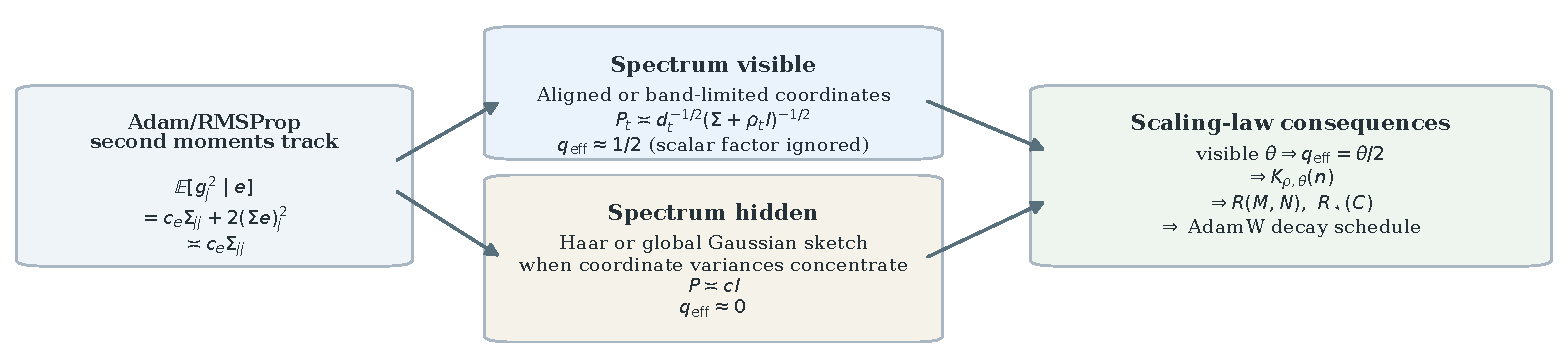
\includegraphics[width=0.96\textwidth]{figures/figure1_visible_spectrum_mechanism}
\caption{Visible-spectrum mechanism. Coordinatewise second moments observe $\diag(\Sigma)$. Aligned or band-limited features yield $\qeff\approx1/2$, whereas globally mixed features yield $\qeff\approx0$. The visible exponent then controls learned modes, risk, compute allocation, and AdamW decay.}
\label{fig:overview}
\end{figure*}

\section{Model, Algorithms, and Scope}

Let $x\sim\mathcal N(0,H)$ and $y=\langle x,w^\star\rangle+\xi$, with $\E\xi=0$ and $\E\xi^2=\sigma^2$.  A feature map $S$ gives trainable features $z=Sx$ with covariance
\[
 \Sigma=\E[zz^\top]=SHS^\top.
\]
This includes eigenbasis coordinates, orthogonal rotations, sketches, and random features.  Excess prediction risk is
\[
 R(w)-\sigma^2=\|w-w^\star\|_\Sigma^2.
\]

\begin{assumption}[Spectrum and source]
\label{ass:power}
The ordered eigenvalues satisfy $\lambda_i(\Sigma)\asymp i^{-a}$ for $a>1$.  If $\Sigma v_i=\lambda_i v_i$, the source energies satisfy
\[
 s_i:=\lambda_i\langle v_i,w^\star\rangle^2\asymp i^{-b},
 \qquad b>1.
\]
For noncommuting preconditioners, the sharp risk theorem uses the corresponding transformed-basis source condition.  Section~\ref{sec:visibility-cases} and the supplement show when it is automatic or holds bandwise.
\end{assumption}

We write $N$ for the number of samples/updates, $M$ for model dimension, and $\Neff=N/\log N$ for the effective horizon of the geometric step-decay schedule used in prior linear-regression scaling theory \cite{lin2024scaling}.  Scalar learning-rate and residual-energy factors are absorbed into $n=\Neff\gamma$ and the damping parameter $\rho$.

For squared loss, with error $e_t=w_t-w^\star$,
\[
 g_t=(\langle z_t,e_t\rangle-\xi_t)z_t.
\]
RMSProp uses $v_{t+1}=\beta_2v_t+(1-\beta_2)g_t^2$ and update
\[
 w_{t+1}=w_t-\gamma_t(v_{t+1}+\epsilon)^{-1/2}g_t.
\]
Adam adds a first-moment EMA, and AdamW additionally applies decoupled shrinkage.

\paragraph{Scope of the sharp theorem.}
The exact transformed-SGD reduction and matching risk law are for a fixed or frozen positive preconditioner.  They extend directly to aligned online dynamics because all coordinatewise preconditioners commute with $\Sigma$ and can be sandwiched by fixed scalar filters.  For general noncommuting online feature systems, Theorem~\ref{thm:visible} is an instantaneous spectral theorem and $\qeff$ is a mechanism diagnostic; we validate its prediction empirically rather than claiming an unrestricted online risk theorem.  This distinction avoids attributing representation-basis effects to a theorem that assumes commutation.

\section{Visible-Spectrum Theory}

\subsection{Actual second moments track coordinate variances}

\begin{lemma}[Gradient second moments]
\label{lem:second-moment}
Conditioned on $e_t$, define $c_t=\sigma^2+\|e_t\|_\Sigma^2$.  Then for every coordinate $j$,
\[
 \E[g_{t,j}^2\mid e_t]=c_t\Sigma_{jj}+2(\Sigma e_t)_j^2,
\]
and therefore
\[
 c_t\Sigma_{jj}\le \E[g_{t,j}^2\mid e_t]\le3c_t\Sigma_{jj}.
\]
\end{lemma}

\begin{proof}
Let $U_t=\langle z_t,e_t\rangle-\xi_t$ and $Z_{t,j}=z_{t,j}$.  Conditionally on $e_t$, $(U_t,Z_{t,j})$ is centered Gaussian with variances $c_t$ and $\Sigma_{jj}$ and covariance $(\Sigma e_t)_j$.  Isserlis' identity gives
\[
 \E[U_t^2Z_{t,j}^2\mid e_t]
 =c_t\Sigma_{jj}+2(\Sigma e_t)_j^2.
\]
The upper bound follows from Cauchy--Schwarz in the $\Sigma$-inner product:
$(\Sigma e_t)_j^2\le\|e_t\|_\Sigma^2\Sigma_{jj}\le c_t\Sigma_{jj}$.
\end{proof}

The population EMA target is
\[
 m_{t,j}=\sum_{s<t}(1-\beta_2)\beta_2^{t-1-s}
 \E[g_{s,j}^2\mid\mathcal F_s],
\]
and let $d_t$ be the same EMA applied to $c_s$.  Lemma~\ref{lem:second-moment} gives
$d_t\Sigma_{jj}\le m_{t,j}\le3d_t\Sigma_{jj}$.

\begin{proposition}[Raw-EMA tracking]
\label{prop:ema}
Let $\Lambda$ be the largest fractional contribution of one sample to any EMA target over $t\le N,j\le M$.  For $\tau\in(0,1/2)$ and failure probability $\delta\in(0,1)$, if
\[
 \Lambda\lesssim \frac{\tau^2}{\log^2(2MN/\delta)},
\]
then, with probability at least $1-\delta$,
\[
 (1-\tau)d_t\Sigma_{jj}
 \le v_{t,j}\le
 3(1+\tau)d_t\Sigma_{jj}
\]
simultaneously over the analyzed horizon.  If $c_t$ changes by at most a factor $\chi$ over the active EMA window, a sufficient condition is
\[
 (1-\beta_2)^{-1}
 \gtrsim \chi\tau^{-2}\log^2(2MN/\delta).
\]
\end{proposition}

The supplement proves Proposition~\ref{prop:ema} using sub-Weibull martingale concentration.  It implies
\[
 (v_{t,j}+\epsilon)^{-1/2}
 \asymp d_t^{-1/2}(\Sigma_{jj}+\epsilon/d_t)^{-1/2}.
\]
The scalar $d_t^{-1/2}$ changes the effective step size; the nontrivial geometry is determined by the coordinate variances.  This is the first link in Figure~\ref{fig:overview}.

\subsection{Visible spectral comparability and the damping transition}

\begin{definition}[Visible exponent]
\label{def:visible}
A normalized diagonal preconditioner $P$ has visible exponent $\theta\in[0,1]$ at damping $\rho$ if constants $0<c\le C<\infty$, independent of scale, satisfy
\begin{equation}
\label{eq:visible}
 c(\Sigma^\theta+\rho I)^{-1/2}
 \pre P\pre
 C(\Sigma^\theta+\rho I)^{-1/2}.
\end{equation}
\end{definition}

\begin{theorem}[Visible-spectrum theorem]
\label{thm:visible}
Under \eqref{eq:visible}, let $\tSig=P^{1/2}\Sigma P^{1/2}$.  Its eigenvalues satisfy
\begin{equation}
\label{eq:effective-spectrum}
 \lambda_i(\tSig)\asymp
 \lambda_i(\Sigma)(\lambda_i(\Sigma)^\theta+\rho)^{-1/2}.
\end{equation}
Consequently, before the damping knee,
\[
 \lambda_i(\tSig)\asymp i^{-\alpha},
 \qquad \alpha=a(1-\theta/2),
 \qquad \qeff=\theta/2.
\]
\end{theorem}

\begin{proof}
The nonzero eigenvalues of $P^{1/2}\Sigma P^{1/2}$ equal those of $\Sigma^{1/2}P\Sigma^{1/2}$.  Congruencing \eqref{eq:visible} by $\Sigma^{1/2}$ sandwiches this matrix between constant multiples of $\Sigma(\Sigma^\theta+\rho I)^{-1/2}$, whose eigenvalues are the right-hand side of \eqref{eq:effective-spectrum}.  The min--max principle completes the proof.
\end{proof}

The damping parameter is not only numerical stabilization.  It sets the spectral range over which adaptivity changes the exponent.  The knee occurs when $\lambda_i^\theta\asymp\rho$, i.e.,
\[
 i_\rho\asymp\rho^{-1/(a\theta)}.
\]
Before the knee, $\tmu_i\asymp i^{-a(1-\theta/2)}$; afterward, $\tmu_i\asymp\rho^{-1/2}i^{-a}$.  The corresponding optimization-horizon knee is
\[
 n_\rho\asymp\rho^{-(1/\theta-1/2)}.
\]

Let
\[
 \Kvis(n)=\#\{i:\lambda_i(\tSig)\gtrsim n^{-1}\}.
\]
For $\theta>0$,
\begin{equation}
\label{eq:learned-count}
 \Kvis(n)\asymp
 \begin{cases}
 n^{1/[a(1-\theta/2)]},
 & n\lesssim n_\rho,\\
 \rho^{-1/(2a)}n^{1/a},
 & n\gtrsim n_\rho.
 \end{cases}
\end{equation}
For $\theta=0$, $K_{\rho,0}(n)\asymp n^{1/a}$.

\subsection{Sharp risk filters}

Let $\tmu_i=\lambda_i(\tSig)$ and $\ts_i$ be transformed source energies.  For a fixed or frozen preconditioner, reduction to SGD on transformed features gives
\begin{equation}
\label{eq:filter-law}
 \begin{aligned}
 \E R_M(w_N)-\sigma^2
 &\asymp \sum_{i>M}\ts_i
 +\sum_{i\le M}\frac{\ts_i}{1+n\tmu_i}\\
 &\quad+\frac1{\Neff}
 \sum_{i\le M}\min\{1,n^2\tmu_i^2\}.
 \end{aligned}
\end{equation}

\begin{theorem}[Visible-spectrum risk law]
\label{thm:risk}
Assume transformed source energies $\ts_i\asymp i^{-b}$ and the clean range $1<b<\alpha+1$.  Then
\[
 \begin{aligned}
 \E R_M(w_N)-\sigma^2
 &\asymp M^{1-b}+\Kvis(n)^{1-b}\\
 &\quad+\frac{\min\{M,\Kvis(n)\}}{\Neff},
 \end{aligned}
\]
up to constants and logarithmic factors.
\end{theorem}

\paragraph{Why the three terms have this form.}
Let $K=\Kvis(n)$.  The approximation tail is
$\sum_{i>M}i^{-b}\asymp M^{1-b}$.  For bias,
\[
 \sum_{i\le M}\frac{i^{-b}}{1+n\tmu_i}
 \asymp
 \frac1n\sum_{i\le K}\frac{i^{-b}}{\tmu_i}
 +\sum_{i>K}i^{-b}.
\]
On an active power-law segment $\tmu_i\asymp i^{-\alpha}$ and $n\asymp K^\alpha$, both terms are $\asymp K^{1-b}$ when $b<\alpha+1$.  For variance, the first $K$ modes contribute $K/\Neff$; the spectral tail is of the same order because
$n^2\sum_{i>K}i^{-2\alpha}\asymp K$ whenever $\alpha>1/2$.  The damped two-slope case follows by splitting both sums at $i_\rho$.  This argument supplies matching lower as well as upper orders, so $K$ is not merely a heuristic effective dimension.

\begin{corollary}[Aligned online RMSProp/Adam]
\label{cor:aligned-online}
Suppose $\Sigma$ is diagonal in optimizer coordinates, Proposition~\ref{prop:ema} holds, $d_t$ stays within fixed positive constants, and the scalar step sizes remain in a stable compact range.  Then online RMSProp has the same learned-mode and risk exponents as the fixed damped profile with $\theta=1$.  Adam with any fixed $\beta_1<1$ has the same exponent, with constants depending on $\beta_1$ and the stability margin.
\end{corollary}

\paragraph{Proof sketch.}
The tracking event sandwiches every diagonal entry of $P_t$ between constant multiples of $(\lambda_i+\rho)^{-1/2}$.  Since all $P_t$ commute with $\Sigma$, every coordinate recursion is bounded by fixed scalar recursions with effective eigenvalues proportional to $\lambda_i(\lambda_i+\rho)^{-1/2}$.  The filter cutoffs and spectral sums therefore agree up to constants.  The momentum statement follows from the characteristic-root calculation below.

\subsection{Compute-optimal allocation and phase transition}

Under compute $C\asymp MN$, the pre-damping proxy is
\[
 \begin{aligned}
 R(M,N,K)-\sigma^2
 &\asymp M^{1-b}+K^{1-b}+K/N,\\
 K&\le N^{1/\alpha}.
 \end{aligned}
\]

\begin{theorem}[Compute-optimal visible scaling]
\label{thm:compute}
Let $m=\max\{\alpha,b\}$, with $\alpha=a(1-\theta/2)$.  Then
\[
 M_\star\asymp C^{1/(m+1)},\quad
 N_\star\asymp C^{m/(m+1)},\quad
 K_\star\asymp C^{1/(m+1)},
\]
and
\begin{equation}
\label{eq:compute-exponent}
 \begin{aligned}
 R_\star(C)-\sigma^2&\asymp C^{-\beta(\theta)},\\
 \beta(\theta)
 &=\frac{b-1}{\max\{a(1-\theta/2),b\}+1}.
 \end{aligned}
\end{equation}
\end{theorem}

For fixed $N$, the unconstrained bias--variance optimum is $K\asymp N^{1/b}$.  If $b\le\alpha$, it exceeds the time cap and $K\asymp N^{1/\alpha}$; this is the \emph{time-limited} phase.  If $b>\alpha$, the unconstrained optimum is feasible and the problem is \emph{variance limited}.  Balancing the optimized $N$ term with $M^{1-b}$ yields Theorem~\ref{thm:compute}.

\begin{corollary}[Visibility phase transition]
\label{cor:visibility-phase}
Let $\theta_c=2(1-b/a)$.  When $0<\theta_c<1$,
\[
 \beta(\theta)=
 \begin{cases}
 \dfrac{b-1}{a(1-\theta/2)+1},
 & 0\le\theta\le\theta_c,\\[6pt]
 \dfrac{b-1}{b+1},
 & \theta\ge\theta_c.
 \end{cases}
\]
Thus visibility improves the compute exponent only until the variance-limited phase; beyond $\theta_c$ it still changes constants and optimal step-size schedules.
\end{corollary}

\subsection{Momentum, AdamW, and hidden-spectrum separation}

For a fixed effective eigenvalue $\mu_i$, Adam first-moment momentum obeys
\[
 e_{t+1,i}
 =
 [1+\beta_1-(1-\beta_1)\gamma\mu_i]e_{t,i}
 -\beta_1e_{t-1,i}.
\]
The slow characteristic root is
$1-\gamma\mu_i+O_{\beta_1}((\gamma\mu_i)^2)$.  Hence momentum changes constants and stability but not the cutoff $N\gamma\mu_i\asymp1$.

AdamW decay $\delta$ gives the exact scalar recursion
\[
 e_{t+1,i}=[1-\gamma(\mu_i+\delta)]e_{t,i}
 -\gamma\delta w_i^\star.
\]
With $w_{0,i}=0$ and $r_i=1-\gamma(\mu_i+\delta)$,
\[
 e_{N,i}
 =-\left[
 \frac{\delta}{\mu_i+\delta}
 +\frac{\mu_i}{\mu_i+\delta}r_i^N
 \right]w_i^\star.
\]
The first term is an irreducible shrinkage floor, so active modes satisfy
$\mu_i\gtrsim\max\{n^{-1},\delta\}$.  If $\delta(C)=C^{-s}$, then
$K\le C^{s/\alpha}$.

\begin{theorem}[Compute-dependent AdamW decay]
\label{thm:adamw}
Let $m=\max\{\alpha,b\}$ and $\delta(C)=C^{-s}$.  The compute-risk exponent is
\[
 \beta_{\rm wd}(\theta,s)=
 \min\left\{\frac{(b-1)s}{\alpha},
 \frac{b-1}{m+1}\right\}.
\]
The no-decay law is recovered iff $s\ge\alpha/(m+1)$.  Fixed positive decay ($s=0$) creates an asymptotic floor.
\end{theorem}


\begin{table}[t]
\centering
\small
\caption{The three Adam components have distinct scaling roles.}
\label{tab:adam-components}
\begin{tabular}{p{0.20\columnwidth}p{0.36\columnwidth}p{0.28\columnwidth}}
\toprule
Component & Mathematical effect & Exponent effect\\
\midrule
Second moment & spectral preconditioner $P_t$ & determines $\qeff$\\
Momentum & stable temporal filter & constants only\\
AdamW decay & cap $\mu_i\gtrsim\delta$ & can reduce exponent\\
\bottomrule
\end{tabular}
\end{table}

Table~\ref{tab:adam-components} clarifies why ``Adam versus SGD'' is too coarse a comparison.  The second-moment geometry is the only component that can alter the spectral power.  Momentum can materially improve transient convergence without changing the asymptotic learned-mode cutoff.  Weight decay can improve finite-sample variance yet eventually hurt scaling if its cap does not move outward with compute.

\begin{proposition}[Tuning cannot close a spectral-exponent gap]
\label{prop:oracle-separation}
Suppose a coordinatewise method has $q_{\rm coord}=0$ while a spectral oracle has $q_{\rm spec}=1/2$.  Define
\[
 \beta(q)=\frac{b-1}{\max\{a(1-q),b\}+1}.
\]
If $\beta(1/2)>\beta(0)$, then
\[
 \frac{R^\star_{\rm coord}(C)-\sigma^2}
 {R^\star_{\rm spec}(C)-\sigma^2}
 \asymp C^{\beta(1/2)-\beta(0)}\to\infty.
\]
Scalar learning-rate tuning changes constants but cannot change this exponent gap.
\end{proposition}

\section{When Is Spectrum Visible?}
\label{sec:visibility-cases}

The same population eigenspectrum can be visible or hidden depending on feature coordinates.  Table~\ref{tab:visibility-cases} summarizes sufficient conditions.

\begin{table*}[t]
\centering
\small
\caption{Feature geometry determines the exponent visible to a coordinatewise optimizer.}
\label{tab:visibility-cases}
\begin{tabular}{llll}
\toprule
Feature geometry & Coordinate variance profile & Effective preconditioner & Predicted $\qeff$\\
\midrule
Eigenbasis aligned & $\Sigma_{jj}=\lambda_j$ &
$(\Sigma+\rho I)^{-1/2}$ & $1/2$\\
Band-limited rotation & band scale $\Lambda_\ell$ &
bandwise spectral, up to constants & $1/2$\\
Controlled profile & $\Sigma_{jj}\asymp\lambda_j^\theta$ &
$(\Sigma^\theta+\rho I)^{-1/2}$ & $\theta/2$\\
Flat/Hadamard & $\Sigma_{jj}=\tr(\Sigma)/M$ &
scalar & $0$\\
Haar/global Gaussian sketch & concentrated quadratic forms &
scalar up to constants & $0$\\
\bottomrule
\end{tabular}
\end{table*}

\paragraph{Aligned coordinates.}
If optimizer coordinates are eigenvectors, then
$P=(\Sigma+\rho I)^{-1/2}$ and $\theta=1$.  Moreover, the transformed target preserves every source energy exactly.

\paragraph{Band-limited mixing.}
Partition eigenvalues into bands $B_\ell$ with
$\kappa^{-1}\Lambda_\ell\le\lambda_i\le\kappa\Lambda_\ell$.
If the feature rotation mixes coordinates only within bands, then every diagonal entry in block $\ell$ is comparable to $\Lambda_\ell$.  Consequently, on that block,
\[
 P_\ell\asymp(\Lambda_\ell+\rho)^{-1/2}I,
\]
and the effective eigenvalues satisfy
$\tmu_i\asymp_\kappa\lambda_i(\lambda_i+\rho)^{-1/2}$.
The exponent is therefore unchanged from the aligned $q=1/2$ case, even though individual eigenvectors are not recovered.

\paragraph{Flat or globally mixed coordinates.}
If
$d_{\min}\le\Sigma_{jj}\le d_{\max}$ with
$d_{\max}/d_{\min}=O(1)$, then
$P\asymp cI$.  Congruence gives
$c_-\Sigma\pre\tSig\pre c_+\Sigma$, so every eigenvalue is preserved up to constants and $\theta=0$.  A normalized Hadamard rotation has exactly flat diagonal.


\begin{proposition}[Exponent-level scalar mixing]
\label{prop:subpoly-mixing}
Let $P_M$ be a sequence of positive diagonal preconditioners with condition number
$\kappa(P_M)=M^{o(1)}$.  If
$\lambda_i(\Sigma_M)=i^{-a+o(1)}$ uniformly on polynomial rank windows, then
\[
 \lambda_i(P_M^{1/2}\Sigma_M P_M^{1/2})
 =i^{-a+o(1)}.
\]
Thus any subpolynomial coordinatewise rescaling has $\qeff=0$ at exponent level, even if it improves finite-size constants.
\end{proposition}

\begin{proof}
Let $p_{\min}$ and $p_{\max}$ be the extreme diagonal entries of $P_M$.  Congruence and the min--max principle give
\[
 p_{\min}\lambda_i(\Sigma_M)
 \le\lambda_i(P_M^{1/2}\Sigma_M P_M^{1/2})
 \le p_{\max}\lambda_i(\Sigma_M).
\]
Because $p_{\max}/p_{\min}=M^{o(1)}$, the multiplicative distortion contributes only an $o(1)$ correction to log--log slopes on polynomial rank windows.
\end{proof}

\paragraph{Gaussian sketches.}
For a Gaussian sketch row $s_j\sim\mathcal N(0,I/D)$,
$d_j=s_j^\top Hs_j$ and $\E d_j=\tr(H)/D$.  A Hanson--Wright bound gives
\[
\begin{aligned}
 &\Pr\!\left(
 |d_j-\tr(H)/D|\ge t\,\tr(H)/D
 \right)\\
 &\qquad\le
 2\exp\{-c\min(t^2\reff,t r_{\rm st})\}.
\end{aligned}
\]
where
$\reff=\tr(H)^2/\tr(H^2)$ and
$r_{\rm st}=\tr(H)/\|H\|_{\rm op}$ \cite{rudelson2013hanson}.
When these ranks dominate $\log(M/\delta)$, a union bound makes the diagonal uniformly flat.  In lower-effective-rank finite problems, the theorem should be treated as a sufficient condition, and measured $\qeff$ determines the actual visible regime.

\section{Experiments}

We report final risk and $\qeff$ separately: final risk captures finite-scale performance; $\qeff$ diagnoses the spectral scaling mechanism.  All stochastic experiments use Gaussian regression with targets constructed in the population eigenbasis to satisfy the source condition.  Learning rates are selected separately for each optimizer and feature geometry.

\paragraph{Protocol.}
The visible-profile run uses dimension $2048$, $(a,b)=(1.5,1.4)$, five trials, mini-batches of size $16$, and checkpoints through $8{,}000$ updates.  Stochastic alignment compares aligned, band-limited, flat, and Haar coordinates with SGD, RMSProp, Adam, AdamW, coordinate oracles, and spectral oracles.  The wide-LR random-feature run uses feature dimension $256$, ambient dimension $2048$, ten trials, $16{,}000$ updates, and adaptive learning rates from $3\times10^{-4}$ to $10^{-1}$.  From the original and effective eigenspectra on the same central rank window, we estimate
\[
 \qeff=1-\widehat\alpha_{\rm eff}/\widehat a.
\]
The supplement proves that this estimator is stable on approximately power-law windows.

\begin{figure*}[t]
\centering
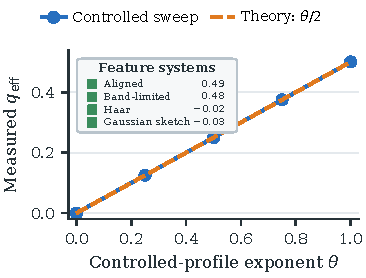
\includegraphics[width=0.32\textwidth]{figures/figure2a_qeff_visibility}
\hfill
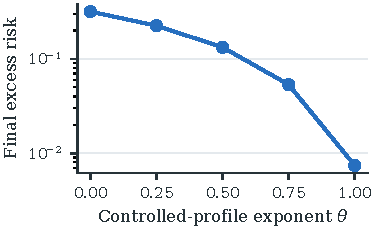
\includegraphics[width=0.30\textwidth]{figures/figure2b_theta_risk}
\hfill
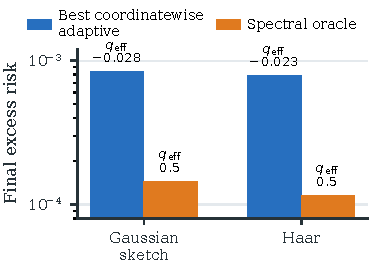
\includegraphics[width=0.32\textwidth]{figures/figure2c_hidden_spectrum_oracle}
\caption{Empirical visibility. Left: measured $\qeff$ follows the visible-profile prediction $\theta/2$. Center: tuned stochastic risk improves as more spectrum becomes visible. Right: under global mixing, a spectral oracle retains $\qeff=1/2$ and lower risk while coordinatewise adaptivity remains near zero.}
\label{fig:experiments}
\end{figure*}

\paragraph{Visible-profile interpolation and robustness.}
Figure~\ref{fig:experiments} summarizes the controlled visibility experiment.  Tuned final risk decreases monotonically from $0.318$ at $\theta=0$ to $0.0074$ at $\theta=1$, while fitted risk slopes steepen from $-0.330$ to $-1.252$.  A separate 20-setting robustness sweep over
$a\in\{1.25,1.5,2,3\}$ and
$\theta\in\{0,.25,.5,.75,1\}$ has maximum errors
$0.00125$ for $\alpha=a(1-\theta/2)$,
$0.00042$ for $\qeff=\theta/2$, and
$0.0131$ for the learned-count exponent.

\paragraph{Damping-knee validation.}
Theorem~\ref{thm:visible} predicts a slope transition at
$n_\rho=\rho^{-(1/\theta-1/2)}$.
Table~\ref{tab:damping} evaluates the exact spectral count far below and above this knee.  Before damping, the learned-count slope depends on $\theta$; after damping, every setting returns to the original SGD slope $1/a=2/3$.

\begin{table}[t]
\centering
\small
\caption{Two-slope damping transition for $a=1.5$.}
\label{tab:damping}
\begin{tabular}{ccrr}
\toprule
$\theta$ & $\rho$ & pre obs./pred. & post obs./pred.\\
\midrule
1.00 & $10^{-8}$ & $1.333/1.333$ & $0.668/0.667$\\
0.75 & $10^{-6}$ & $1.065/1.067$ & $0.671/0.667$\\
0.50 & $10^{-3}$ & $0.882/0.889$ & $0.676/0.667$\\
\bottomrule
\end{tabular}
\end{table}

\paragraph{Alignment, source diagnostics, and online adaptive methods.}
Actual RMSProp/Adam/AdamW second moments have
$\qeff\approx0.48$--$0.51$ in aligned and band-limited coordinates, but $\qeff\approx0$ in flat/Haar coordinates.  This split persists after optimizer-specific learning-rate tuning.  Source diagnostics show exact exponent preservation for aligned and scalar-preconditioned cases, exact blockwise mass preservation under band-limited rotations, and the expected basis-dependent variation under global mixing.  These checks separate a spectral failure from a source-condition failure.

\paragraph{Random features and sketches.}
Table~\ref{tab:random-feature} reports the difficult globally mixed cases after the wide LR grid.  Coordinatewise Adam/RMSProp have $\qeff\approx0$, while a spectral oracle retains $\qeff=1/2$ and achieves substantially lower risk.  Global mixing therefore hides useful spectrum from diagonal adaptivity; it does not eliminate the spectrum itself.

\begin{table}[t]
\centering
\small
\caption{Wide-LR random-feature results.}
\label{tab:random-feature}
\setlength{\tabcolsep}{3pt}
\begin{tabular}{@{}llrr@{}}
\toprule
Case & Optimizer & Final risk & $\qeff$\\
\midrule
Gaussian sketch & Adam & $8.35\!\times\!10^{-4}$ & $-0.028$\\
Gaussian sketch & RMSProp & $1.52\!\times\!10^{-3}$ & $-0.032$\\
Gaussian sketch & Spectral oracle & $1.45\!\times\!10^{-4}$ & $0.500$\\
Haar & AdamW & $7.84\!\times\!10^{-4}$ & $-0.023$\\
Haar & RMSProp & $9.50\!\times\!10^{-4}$ & $-0.027$\\
Haar & Spectral oracle & $1.16\!\times\!10^{-4}$ & $0.500$\\
\bottomrule
\end{tabular}
\end{table}

\paragraph{Compute and weight decay.}
Figure~\ref{fig:compute} shows the compute and AdamW phase diagrams.  In a hard-source case $(a,b)=(3,1.4)$, the observed compute-risk exponent improves from $0.102$ at $\theta=0$ to $0.167$ at $\theta=1$, closely matching predictions $0.100$ and $0.160$.  In a saturating case, the exponent plateaus after the predicted phase boundary.  AdamW schedule sweeps verify that $\delta(C)=C^{-s}$ recovers the no-decay law exactly when $s\ge\alpha/(m+1)$.

\begin{figure*}[t]
\centering
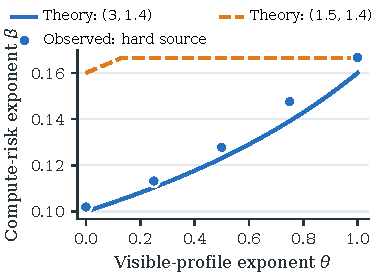
\includegraphics[width=0.32\textwidth]{figures/figure3a_compute_phase_transition}
\hfill
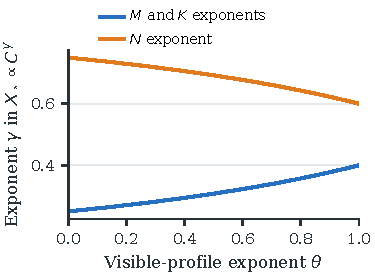
\includegraphics[width=0.32\textwidth]{figures/figure3b_allocation_exponents}
\hfill
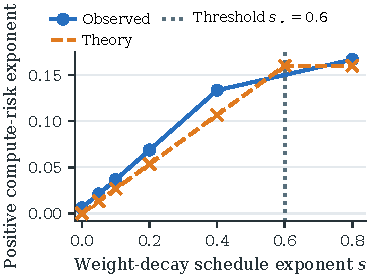
\includegraphics[width=0.32\textwidth]{figures/figure3c_adamw_schedule}
\caption{Compute and AdamW phase diagrams. Left: observed compute-risk exponents track the visibility-dependent theory. Center: optimal model, data, and learned-mode allocation exponents vary with $\theta$. Right: the AdamW decay schedule recovers the no-decay exponent only after the predicted threshold.}
\label{fig:compute}
\end{figure*}


\section{Interpretation and Testable Predictions}

The visible-spectrum viewpoint turns several empirical optimizer questions into geometric predictions.

\paragraph{Block structure should matter.}
A diagonal method can use only the spectrum encoded in coordinate variances.  A matrix or block preconditioner can rotate into a more informative basis.  The band-limited theorem therefore predicts that Shampoo- or SOAP-style blocks help most when each block spans a narrow spectral range; mixing unrelated scales inside a block should wash out the gain.  This complements recent observations that blocking and explicit spectral normalization improve hyperparameter transfer for matrix-preconditioned optimizers \cite{vyas2024soap,qiu2025hyperparameter}.

\paragraph{Optimizer constants and optimizer exponents should be reported separately.}
A larger stable step size can yield a dramatic finite-budget improvement while leaving $\qeff=0$.  Conversely, a true exponent improvement may look modest at small scale but compound with compute.  A robust optimizer comparison should therefore report: tuned risk, the effective spectral slope, the transformed source profile, and whether the fitted range lies before or after the damping knee.  Proposition~\ref{prop:oracle-separation} explains why learning-rate tuning cannot eliminate a genuine exponent gap.

\paragraph{Damping and weight decay must scale with the training regime.}
The numerical stabilizer $\epsilon$ determines $\rho=\epsilon/d_t$ and hence the extent of the pre-damping regime.  Fixed $\rho$ eventually returns the learned-count slope to $1/a$ even when $\theta>0$.  AdamW decay introduces a second, independent ceiling.  Consequently, an optimizer can exhibit an adaptive exponent at moderate scale yet revert or saturate at larger scale if $\epsilon$, residual normalization, or weight decay is held fixed.  This offers a mechanistic explanation for apparently inconsistent cross-scale optimizer comparisons.

\paragraph{Deep networks admit a layerwise diagnostic.}
Our linear theory does not assign one global $\theta$ to a neural network.  It instead suggests measuring a layerwise or blockwise visible exponent from the covariance and second-moment preconditioner at several checkpoints.  If representations become more globally mixed during training, $\theta$ should fall; if feature learning aligns coordinates with task-relevant eigendirections, $\theta$ should rise.  These predictions are falsifiable without fitting a full end-to-end neural scaling law.


\section{Related Work}

\paragraph{Empirical and theoretical scaling laws.}
Empirical scaling laws span language modeling, generative modeling, and transfer
\cite{hestness2017deep,rosenfeld2020constructive,kaplan2020scaling,henighan2020scaling,hernandez2021scaling,hoffmann2022training}.
Later work also documents broken or nonmonotone regimes \cite{caballero2023broken}.
Spectral accounts connect power laws to kernel eigenvalues, task alignment, and overparameterized regression
\cite{bordelon2020spectrum,canatar2021spectral,bahri2021explaining,simon2024more}.
The closest theoretical baseline is the sharp one-pass SGD theory of
\citeauthor{lin2024scaling} (\citeyear{lin2024scaling}).
Subsequent work studies data reuse and mini-batching
\cite{lin2025datareuse,chen2026minibatch}.
We keep the same power-law regression laboratory but make optimizer geometry the object of study.

\paragraph{Optimizer-dependent scaling and hyperparameter transfer.}
Recent random-feature experiments directly report optimizer-dependent scaling exponents \cite{ramani2026optimizer}; our work provides a complementary theorem that identifies when a coordinatewise optimizer can realize such an exponent shift.
At larger scales, reliable optimizer comparison also requires hyperparameters that transfer across width and depth.  Maximal-update parameterization and recent matrix-preconditioner studies show that incorrect learning-rate or weight-decay scaling can erase apparent gains
\cite{yang2022tensor,qiu2025hyperparameter}.
This motivates our optimizer-specific LR grids and the explicit AdamW decay theorem.

\paragraph{Adaptive and matrix preconditioning.}
Adaptive optimization includes AdaGrad and RMSProp
\cite{duchi2011adaptive,tieleman2012rmsprop}, as well as Adam and AdamW
\cite{kingma2015adam,loshchilov2019decoupled}.
Prior theory studies convergence and generalization
\cite{reddi2018convergence,wilson2017marginal}, together with optimizer-dependent implicit bias
\cite{zhang2024implicit,vasudeva2025rich}.
Natural gradient, K-FAC, Shampoo, and SOAP make matrix or rotated-basis preconditioning explicit
\cite{amari1998natural,martens2015optimizing,gupta2018shampoo,vyas2024soap}.
Our distinction is geometric: scalar normalization can improve constants, whereas a change in spectral power changes the scaling-law class.

\paragraph{Random features, sketches, and high-dimensional regression.}
Random features and kernel approximations provide tractable models of representation geometry
\cite{rahimi2007random,rudi2017generalization,bach2017breaking,jacot2018neural}.
Benign overfitting and double descent expose the role of spectral tails and effective dimension
\cite{belkin2019reconciling,bartlett2020benign,hastie2022surprises}.
Our results add a basis-sensitive layer: the same covariance eigenvalues can be visible to a spectral or band-aware optimizer but hidden from a coordinatewise optimizer after global mixing.

\section{Limitations and Conclusion}

The analysis is for Gaussian linear regression and related feature-coordinate models.  Neural networks have non-Gaussian gradients, evolving representations, normalization layers, and optimization--representation interactions.  The visible-spectrum condition is a sufficient description of optimizer geometry; it does not assert that every network layer has a fixed $\theta$.  Our sharp online risk corollary also requires aligned commuting dynamics.  In general feature systems, we use $\qeff$ as a diagnostic supported by experiments.

These limitations also suggest concrete next steps.  The theory predicts that layerwise or blockwise adaptive methods should benefit when their blocks align with narrow spectral bands, and that optimizer gains should weaken when normalization or feature mixing flattens coordinate variances.  Both predictions are measurable in deep networks by logging second-moment preconditioners and effective spectra.

Adaptive optimizers do not automatically change scaling laws.  They change spectral exponents when their coordinatewise second moments reveal covariance structure.  The visible exponent $\theta$ determines $\qeff$, the learned-mode count, compute allocation, and AdamW decay schedule.  This provides a precise criterion for when optimizer choice should enter scaling-law forecasts.

\bibliography{references}

\end{document}
